\section{Galaxies}

\begin{sectionauthor}
     Mandy Chen (The University of Chicago) \\
     Ava Polzin (The University of Chicago) \\
     Zili Shen (Yale University)
\end{sectionauthor}
\vspace{20pt}

\subsection{Morphology and Classification}

Galaxies have traditionally been classified based on their morphology (their shape) and size. There are three major types of galaxies (by shape) -- spirals (characterized by their disk-like shape and clear substructure), ellipticals (generally more diffuse with little-to-no substructure), and irregulars (which are a catch-all class that incorporates low mass galaxies, galaxies actively undergoing mergers, etc.). Galaxies can also have various morphological features, like bars or rings, that can play into the characterization.

There is also a mass/size-based distinction. Dwarf galaxies have stellar masses that are (roughly) $10^4 - 10^9 \times$ the mass of the sun (ultra-faint dwarf galaxies -- named for their incredibly low luminosities -- are generally in the $10^4 - 10^5$ solar mass range, while galaxies that are millions to billions of times the mass of the sun are often referred to as ``classical'' dwarf galaxies). Ultra-diffuse galaxies are characterized by their dwarf-like masses and physical sizes that are more consistent with more massive galaxies, making them more diffuse (as the name suggests). Massive galaxies generically refer to galaxies with stellar masses $\gtrsim 10^{10}$ solar masses. L$^*$ galaxies refer to galaxies that exist at the knee of the Schechter luminosity function, which shows the number density of galaxies as a function of their intrinsic brightness, and are approximately the same mass (and so approximately the same brightness) as the Milky Way galaxy. Though L$^*$ galaxies are often considered ``typical'' galaxies, they actually represent an expansive, heterogeneous population, with a variety of physical and chemical characteristics.

Because of the finite speed of light, when we look at very distant (high redshift) galaxies, we are looking at galaxies in earlier stages of their evolution. It is common to assume that the galaxies observed at high redshift are analogs for the progenitors of modern day galaxies, so this is an avenue for us to understand how galaxies grow and change with cosmic time.

There's a strong connection between a galaxy's size and its intrinsic brightness. More massive galaxies generally have more stars, making them more luminous. The type of stellar population also makes a difference -- younger stellar populations with massive and luminous (but very short-lived) stars will be brighter than older stellar populations in which these very bright young stars have died off. This connection is one of the ways astronomers use the light observed from galaxies to infer their masses -- if you know the distance, and so the intrinsic brightness, and can make some assumptions about the population of stars, you can estimate the galaxy's stellar mass. Of course this isn't the only mass component in galaxies. They also include gas (which is not optically luminous, but can emit at other wavelengths when ionized) and dark matter, discussed more in the rest of this section. This also means that low mass galaxies (whether local dwarf galaxies or high redshift galaxies that are still forming) are exceptionally difficult to observe due to their intrinsically low luminosities.

\begin{figure}
    \centering
    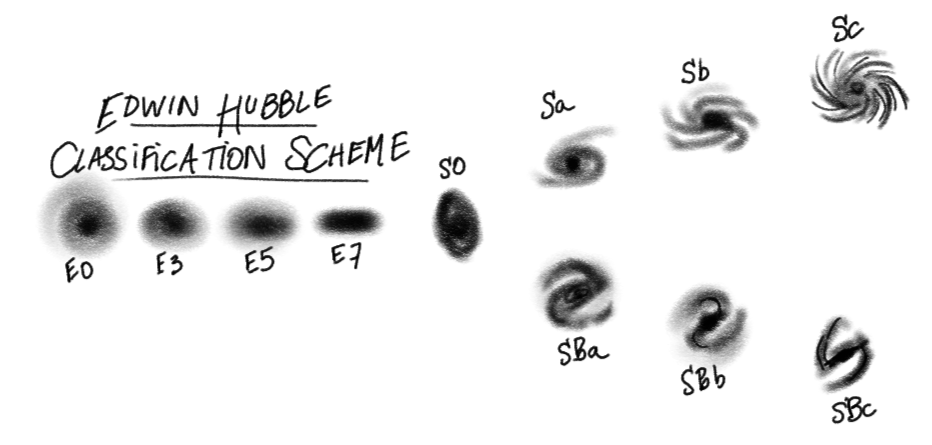
\includegraphics[width=0.8\linewidth]{img/galaxyclass.png}
    \caption{Edwin Hubble's original galaxy classification scheme, sometimes called the ``Hubble tuning fork''. While not all galaxies are well-described by the \textit{elliptical}/\textit{spiral} dichotomy, and it doesn't take all galaxy properties into account and is only based on optical light, the tuning fork still forms the basis of how we describe galaxies in many cases today.}
    \label{fig:galaxyclass}
\end{figure}

\subsection{Distance Estimation}

One of the biggest challenges in discerning a galaxy's properties comes from needing to understand how far away it is to convert between observed properties and intrinsic properties. Without accurate distance estimates, we don't know how bright, how large, or how massive a galaxy is -- we can't even accurately infer anything about a galaxy's immediate environment without constraints on its distance.

Because different distance measurements are useful for objects that range from the very local -- astronomically speaking -- to the very distant, the different measurement methods are referred to as the cosmic distance ladder. The first rung is useful in our immediate neighborhood.

Very locally, when looking at stars in our own Galaxy\footnote{The Milky Way is often denoted Galaxy with a capital ``G'', while galaxy as a generic term is written in lower case.}, we can use the immensely accurate parallax distance. Parallax takes advantage of the changing viewing position of an observer (we can do this on large scales given the Earth's changing position over the course of a year -- two observations six months apart will have the largest baseline displacement) to infer distance from the changed apparent position of the measured object. You can test this yourself. Hold your hand at arm's length and point your finger -- close your non-dominant eye and observe where your finger is pointing. Now, without changing where you are pointing, switch which eye is open; you'll find that, from the perspective of this eye, you are now pointing at a different object. Now bring your finger closer to you and do the same. In which case does your pointed finger end up appearing to move more? The closer one, right? That is because distance ($d$) is proportional to the inverse of the parallax angle ($p$) -- $d \propto 1/p$. This can be worked out directly if $p$ is measured in arcseconds and $d$ is measured in parsecs. The problem is, for large enough distances, you need a sufficiently large baseline to measure any perceptible difference in $p$. This means that extragalactic distances have to be measured differently.

The first extragalactic rung  on the distance ladder is generally the relationship between the light curves of Cepheid variable stars (which show fluctuations in brightness with time as their radii and temperature change) and their intrinsic brightness. Henrietta Swan Leavitt, one of the famous female astronomers that worked at the Harvard Observatory during the early 20th century, discovered that there was a tight correlation between the period of this variability (the period is the time between two peaks or two troughs in the light curve) and the luminosity of the variable star. Since the period can be observed and measured without knowing anything about the distance, this relationship allows us to infer the distance because the luminosity, $L$, is related to the observed brightness $F$ by $L = 4\pi d^2 F$, so $d = [L/(4\pi\, F)]^{1/2}$. In effect, the Leavitt Law, as it is now known, allows Cepheid variable stars to act as ``standard candles''. At slightly greater distances, you can use Type 1a supernovae as standard candles if you're lucky enough to have observed one that is reliably linked to a host galaxy. 

``Tip of the red giant branch'' (TRGB) distance measurements use the same principle -- the intrinsic brightness of the most luminous red giant stars is well understood and can be used to then infer the distance to the galaxy. This requires that there is a \textit{resolved} image of the galaxy, where we can distinguish, and measure the brightness from, individual stars. Unfortunately, even with Hubble and JWST, this places an upper limit on the distance out to which we can reliably infer a TRGB distance. A similar effect that we use to determine distance is from ``surface brightness fluctuations'' (SBF). SBF distances rely on the fact that, for a particular telescope, a stellar population will get less and less resolved at greater distances -- we can then use the pixel-to-pixel variation of the images as a proxy for how resolved the stellar population is. A less resolved galaxy will have less pixel-to-pixel variation than a fully resolved galaxy.

Each of those methods relies on imaging, but we can also use spectroscopic measurements to estimate how far away a galaxy is. Taking spectra is very expensive and very time intensive compared to imaging the sky, but ``if a picture is worth one thousand words, a spectrum is worth one thousand pictures.'' If a galaxy is sufficiently far away, so that its velocity is primarily attributable to the Hubble flow (the speed at which the universe is expanding) rather than random motions (the galaxy's peculiar velocity) or interaction with large scale structure, we can infer a distance based on the line-of-sight velocity (also called the radial velocity). Redshift, a term you have probably heard before in this context, is generally just $z = v/c$, where $v$ is the radial velocity and $c$ is the speed of light. We can measure where various spectral lines are relative to where we expect them to be, which gives us $z$. For a single assumed expansion speed of the universe, there is a distinct distance that is related to a galaxy's measured redshift. In addition to getting a distance estimate, spectra give us a tremendous amount of detailed information about the chemical and physical characteristics of the observed galaxy. Spectra are then critical for all sorts of galaxy studies. 

\vspace{-10pt}

\subsection{Star Formation}

Baryons are the ``normal'' (i.e., not dark) matter in galaxies, so when astrophysicists refer to the baryon cycle, we are talking about the way that gas forms stars, is recycled into the galactic environment, and so-on.

Cold, dense gas, when it gets cold and dense enough, coalesces to form stars. These stars can live a very long time (as with low mass stars) or a very short time (as for extremely luminous, massive stars). This gas that formed stars is then partially locked in old stars and partially recycled into the gas in and around the galaxy by the end stages of stellar evolution. When these massive young stars go supernova, the enriched material from their inner layers (replete with heavy elements due to the fusion that takes place in stellar cores) is blown away from the stellar remnant and into the galaxy's gaseous medium. Some of this gas will end up back in a new generation of stars after it has cooled and coalesced and some will end up in the galaxy's halo. Cold gas can also be accreted onto the galaxy (or brought in due to gravity) from the galaxy's surroundings. These processes make up the baryon cycle.

Because you need cold neutral gas to form stars, star formation can shut off when the galaxy's reservoir of gas becomes ionized or heated (from the presence of bright young stars, supernovae, or due to interactions with neighboring galaxies). When star formation shuts off, it's called quenching, and the exact processes that quench some galaxies are poorly understood, particularly for very low mass galaxies and those at high redshifts. A new generation of instruments (including JWST, the Vera C. Rubin Observatory, and some exciting upcoming telescopes like the Nancy Grace Roman Space Telescope) and simulations are enabling us to begin looking into these questions in more detail.

We can infer the amount of active star formation in a galaxy several ways, though perhaps most notably from the light of young stars (generally in the far ultraviolet) or from the presence of gas that has been ionized by young, massive stars (the H$\alpha$ line at 6563\AA~is typically used, though there are other tracers). In addition to understanding how much immediate star formation is occurring (in the last 5 - 100 Myr depending on the selected tracer), we can also access the star formation history of a galaxy since the light in images and spectra is made up of many generations of stars. Using spectral energy distributions (SEDs), which look at the amount of flux across wavelengths, we can better understand when star formation occurred in the galaxy and how it evolved over time -- i.e., were all of the stars formed in a single burst, was there constant star formation across a period, or does the star formation history look different than either of these scenarios? Combining multi-wavelength photometry with spectroscopy gives us a more detailed star formation history than looking at the brightness of an image in one filter or the strength of a single spectral line, since it is anchored on so many individual data points. The calibrations that underlie these methods are generally done empirically, where we have many observations (across the electromagnetic spectrum) that allow us to describe how an observed parameter is connected to the galaxy's properties, while theory can help us pinpoint the exact relationships between tracers. There are still uncertainties, though, particularly as we reach new parts of the observational parameter space, like the extremely high-redshift galaxies being observed for the first time with JWST.

\subsection{Star Clusters \& Stellar Streams}
Most stars in a galaxy are distributed smoothly but not uniformly: the stars are denser in the middle of the galaxy and less dense towards the outskirts. Multiple generations of stars form and disperse in the galaxy, making it hard to disentangle their origins. However, some stars form together and stay together in a cluster because they are gravitationally bound to each other. Star clusters not only look spectacular but also provide key tools for studying galaxies.

We observe two types of star clusters in the present-day universe: open clusters and globular clusters. Pleiades (colloquially known as the Seven Sisters) is an open cluster. These clusters are young, but we know that going forward, they will likely disperse in several million years. Globular clusters, on the other hand, are ancient. They can wander through the host galaxy for ten billion years (except in extreme situations, see stellar streams). They can survive so long because they are dense: millions of stars crowd together inside several parsecs. The progenitors of globular clusters cannot be open clusters because of the age mismatch. JWST has observed “proto-globular-clusters” in high-redshift galaxies, which is the first time that we can study globular cluster formation with observations.

Star clusters and dwarf galaxies can stretch into stellar streams when they fall into a much more massive galaxy. When the external gravitational force from the colliding galaxies exceeds the gravitational pull of the stars inside the cluster, the cluster starts to dissolve into a ribbon-like river of stars called a stellar stream. The stars stay in the stream not due to any physical forces but due to their coherent motion. The motion of these stars is governed by the combined gravity of the massive galaxy and its progenitor, and any close encounters with massive objects can send stars flying off and create a gap in the stream. Thinner streams are more sensitive to these perturbations, making them the ideal tracer of the galactic potential and any substructures within.

\subsection{Dark Matter}
Even though we are most familiar with things composed of atoms and molecules, this type of matter (baryonic matter) only accounts for 15\% of all matter in the Universe. The other 85\% is what we call dark matter. Dark matter doesn’t emit or reflect light, but it does exert gravity on everything else in the Universe. That’s a strange theory about our Universe, you may say. How do we know there exists something that we can’t ever see?

For that, we must thank Vera Rubin for her work on galaxy rotation curves. She was the first female astronomer to observe at the Palomar Observatory in 1965, which had only allowed men until then. She discovered that the outer parts of galaxies rotate as quickly as components closer to the center. That implies that the enclosed mass in the galaxy keeps growing towards the outside, even beyond where stars and gas are observed. The missing mass then became key evidence for the existence of a ``dark matter halo'' in every galaxy. The dark matter would account for over 95\% of the total mass in a galaxy, with only 5\% in stars and gas. Dark matter is a key ingredient in modern galaxy formation theory. Dark matter halos are the sites where galaxies form: their gravity attracts gas which then collapses and forms stars. 

As important as dark matter is in astrophysics, we still don’t have conclusive evidence of what it is. The most widely accepted candidate is Cold Dark Matter, which hypothesizes that dark matter is a particle that moves slowly compared to the speed of light, and that it does not interact with electromagnetic radiation (light). This is the simplest explanation for all the observational evidence, but this particle hasn’t been directly detected despite our best efforts. This leaves room for other types of dark matter, and modified gravity, which are alternative theories to explain the missing mass in galaxies. These theories all make different predictions about properties of galaxies, so astrophysical observations can distinguish between these models in the future.

One example of this is the recent discovery of galaxies that lack dark matter. This is somewhat surprising given the standard theory that galaxies form inside dark matter halos. Thus, these “dark-matter-deficient galaxies” have been extensively observed. There are some astrophysical routes to remove dark matter from existing galaxies (such as tidal stripping, see paragraph on stellar streams), and there are also ways to form exotic galaxies without dark matter (such as a high-speed collision of progenitor galaxies). The recent discoveries support a dark matter particle instead of modified gravity.


\subsection{Gaseous Environments \& Turbulence}
Observations of galaxies, particularly imaging data such as the beautiful pictures from state-of-the-art telescopes (e.g., {\it Hubble Space Telescope} and {\it James Webb Space Telescope}), are dominated by the continuum radiation from stars. While our eyes are naturally drawn to these bright regions of a galaxy, the dominant component that makes up the majority of a galaxy's baryonic mass actually exists in a tenuous gas phase. This low-density gas (with a density as low as $\sim0.0001$ particles per cm$^3$) can extend much beyond the visible stellar disks/bulges and into the circumgalactic and intergalactic space. Generally, people call this diffuse gaseous structure circumgalactic medium (CGM) if it's gravitationally bound to a galaxy or intergalactic medium (IGM) if it's not clear which galaxy the gas belongs to, although in practice the definitions are less well-defined and the boundary between the CGM and IGM is not always clear. 

The IGM and CGM play a critical role in driving galaxy formation, maturation, and eventual quiescence. Star formation consumes the gas inside a galaxy and if left without replenishment, star formation cannot continue and a galaxy will stop from growing further, which is in contradiction to observations that show continuous growth via star formation in many galaxies. Therefore, a key component in modern galaxy evolution models is the presence of gas accretion from the IGM and CGM that serves as the fuel to sustain star formation.  At the same time, activities due to star formation and active galactic nuclei (i.e., active supermassive black holes at the center of galaxies) can inject a large amount of energy and materials back into the CGM and IGM through energetic processes such as galactic outflows. Through depositing energy and materials outside of the star-forming regions, galaxies exhibit suppressed star-formation rates.  Gas accretions/infalls are commonly called {\it feeding} while processes like outflows are called {\it feedback}. As feeding and feedback have the opposite effects on galaxy growth, the intricate interplay between these two processes dictates the cosmic star formation history. Therefore, it is of great interest for us to understand the properties of the CGM and IGM, and in general the gaseous environments both inside and surrounding galaxies, in order to improve our theories of galaxy evolution.


\begin{figure}
    \centering
    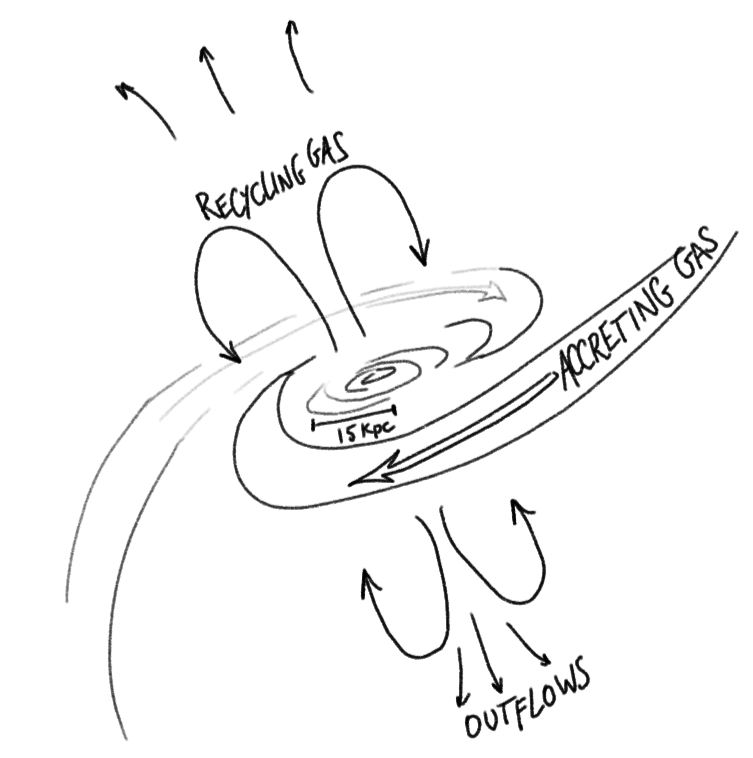
\includegraphics[width=0.75\linewidth]{img/galaxy_outflow.png}
    \caption{The in/outflow of gas on galaxy scales involves a number of processes internal to the galaxy and is informed by the galaxy's environment.}
    \label{fig:galaxy_outflow}
\end{figure}

As mentioned above, the gas density of CGM and IGM is typically extremely low.  As a result, for the past few decades, observations of this tenuous gas have largely relied on a technique called {\it absorption spectroscopy}. This technique uses the light emitted by a bright background source at large distances (most commonly a supermassive black hole that's actively accreting mass from its surroundings and emitting an enormous amount of energy in radiation) and looks for absorption features in the spectrum of this background source.  The absorption is caused by intervening low-density gas between us, the observer, and the background light source. The shapes and intensity of the absorption features can tell us about many physical properties of the gas, such as density, temperature, kinematics, metallicity, and ionization state. A complementary method of observing the CGM and IGM is to directly detect the light emitted by the gas. However, because of its tenuous nature, such emission is extremely faint and has been mostly impossible to detect until the recent advent of high-throughput integral field spectrographs on large ground-based telescopes, such as the Multi Unit Spectroscopic Explorer (MUSE) on the Very Large Telescopes (VLT) and the Keck Cosmic Web Imager  (KCWI) on the Keck Telescopes. These integral field spectrographs have unrivaled sensitivity to faint emission signals and their data have recently constituted the new frontier for CGM and IGM research. With an IFU, each pixel provides a spectrum in what is called a data cube -- this allows for sensitive, spatially resolved information about the gas composition and velocity.

In addition to its low density, one particularly interesting aspect of the CGM and IGM gas is its turbulent nature.  Because the gas typically moves at a large velocity in space, we expect the gas to be turbulent.  This means that the gas motions are chaotic and have little coherency from one location to the next (in contrast to, for example, the water flowing out of a faucet). The presence of turbulence in the diffuse halo gas and the degree of such turbulence have profound implications for the thermal and dynamic properties of the CGM and IGM. Turbulent energy can be a significant source of heating to offset energy lost due to radiation.  Turbulence can also provide additional pressure support in the gas halos and prevent them from collapsing under gravity. In addition, turbulence produces density fluctuations, triggering and facilitating the formation of gas structures in different temperature phases. Turbulent mixing also provides an efficient transport mechanism for metals from star-forming regions to the CGM and IGM.